% Deployment chapter continued
\section{Infrastructure from 5,000 feet}
Figure \ref{fig:infra5k} shows the final assembly of whirlpool crawler project. 
\begin{figure}[h!]
  \centering
  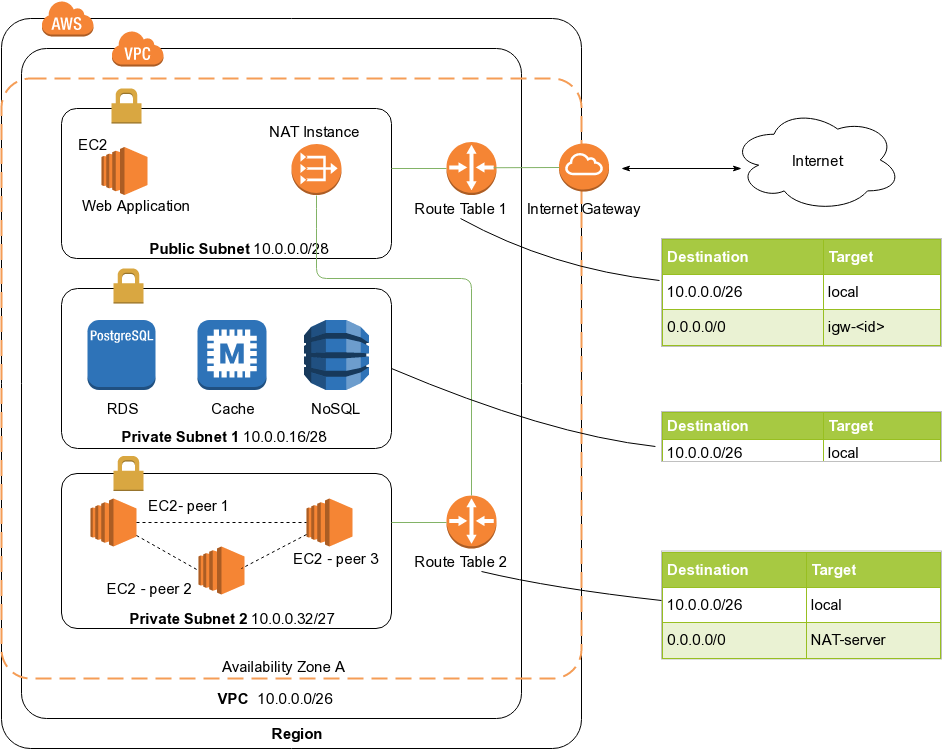
\includegraphics[width=20cm,height=12cm,keepaspectratio]{../media/crawler/aws-deploy-5k-feet.png}
  \caption{Whirlpool infrastructure with Route tables, NAT}
  \label{fig:infra5k}
\end{figure}

\noindent
Each subnet gets assigned a main route tables which cannot be deleted but instead can be overridden with custom route tables immediately effective on subnets as evident in figure \ref{fig:infra5k} with route tables 1 \& 2. Speaking of NAT instance in public subnet 1, is like any other AMI linux image but ships with pre-configured iptables. NAT forwards traffic from instances in subnet 4 to the internet and send the response for corresponding request back to those instances in subnet 4. It won't allow outside clients to initiate connections with instances in subnet 4. The custom route(shown in route table 2) directs the traffic originated within any of the private subnet peers matching subnet mask \ipAddress{0.0.0.0/0} to NAT server. The custom route(show in route table 1) scopes all packets matching \ipAddress{0.0.0.0/0} route to IGW. The traffic from private crawler subnet flows to NAT Instance and then to the IGW. The NAT translate back-and-forth source and destination IPs of private instances assuming external property - source/destination check is disabled.
\\
\\
\noindent
The subsystems of whirlpool leverage relational database(Amazon RDS) to maintain a history of URLs, NoSQL(EC2-mongoDB) to store extracted text. AWS does not have managed instance of MongoDB and requires the interested party to operate, maintain on an EC2 Instance. Also, later on, a cache server(AWS ElasticCache) can be adopted to optimize lookup efficiency against relational database by those subsystems dependent on it. Given this requirement, its safer to form a private subnet 2 dedicated to placement of data stores and in-memory cache as shown in the figure \ref{fig:infra5k}. This way, the data store subnet would stay safer accepting network connections within the VPC, specifically only from instances allowed by statefull firewalls(VPC security groups) attached to it. For relational database, amazon's RDS DB subnet group mandates 2 subnets, each in different availability zones to successfully launch the instance. Thus, a private subnet 3 in the figure.

\pagebreak

% note - here expand on EC2, RDS, cache, NoSQL, NAT computing specifications
\section{AWS Services Hardware Specfication \& Cost Estimation}

\begin{figure}[h!]
  \centering
  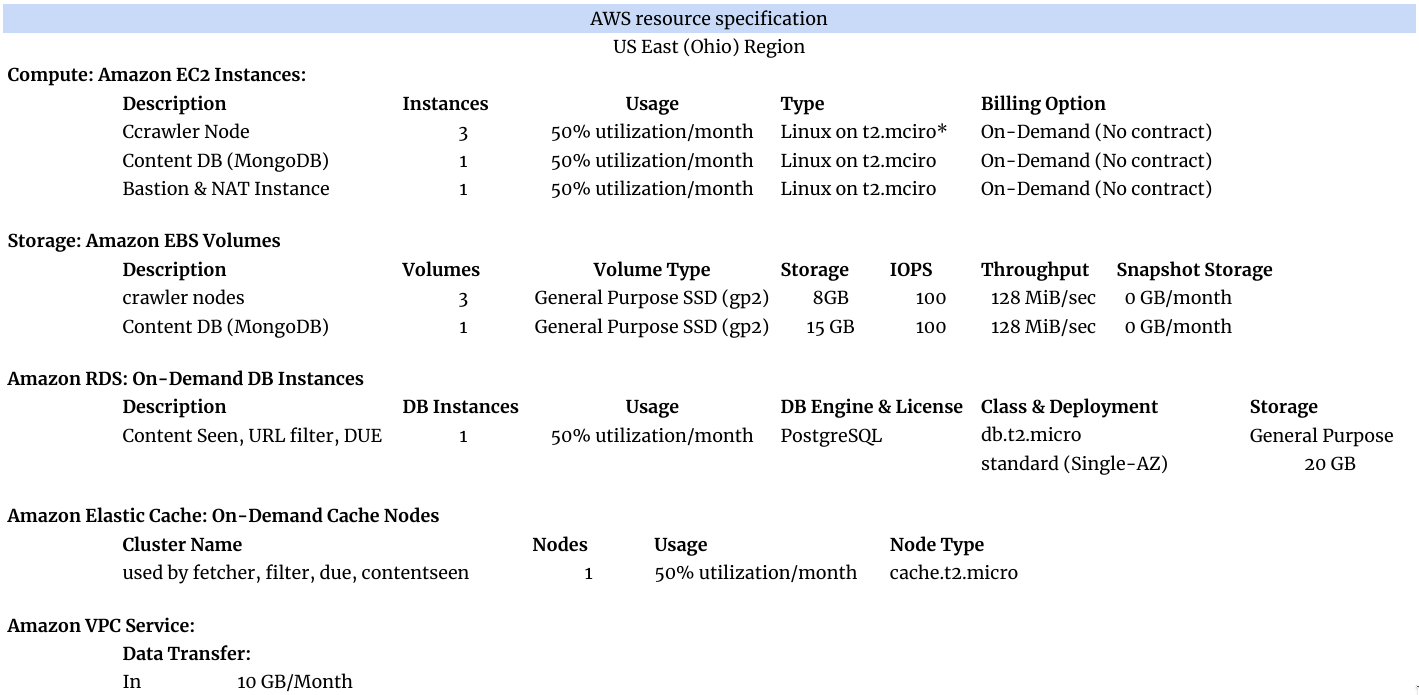
\includegraphics[width=16cm,height=13cm,keepaspectratio]{../media/crawler/aws-resource.png}
  \caption{Whirlpool Hardware Specification on AWS}
  \label{fig:awsspec}
\end{figure}

\noindent
From table \ref{fig:awsspec} under Amazon EC2 services, a crawler node sits on a on-demand EC2 instance which is of type t2.micro. The t2.micro has single core virtual CPU (vCPU) with 1 GiB of Memory. Each crawler node runs a message broker - RabbitMQ to interconnect the crawler subsystems. According to RabbitMQ Documentation
\cite{rabbitmq}, the host should have at least 128 MB memory available at all times. Moreover, it wont accept
any new messages when it detects that its using more than 40\% of avialable memory. Being said that, there is
always an option to change the current instance type from t2.micro to t2.small and so on depending on
usage. MongoDB which collects extracted text is hosted on On-Demand t3.micro instance type, which is a 1 GB, dual-core vCPU operating at 50\% of its capacity.
\\
\\
\noindent
Coming to Amazon Storage,  the crawler node is coupled with Elastic Block Storage(EBS) volume of 5 GB. The volume is general purpose SSD capped at 100 IOPS giving a throughput of 128 MB/sec. For mongoDB an EBS volume
of 15GB is used. It is formatted with XFS filesystem for its data directory as recommended in its production checklist.
\\
\\
\noindent
Whirlpool uses one On-Demand RDS instance with PostgreSQL engine operating at 50\% utilization monthly. The underline managed Operating System is a db.t2.micro deployed in a single AZ. PostgreSQL to store fingerprints of a web page content at a given URL, robots.txt attributes of each site, and URLs already enqueued to be crawled.
\\
\\
Amazon ElasticCache provides a choice between Memcached \& Redis Instance. It will be used by URL filter
subsystem of whirlpool.
\\
\\
Lastly, Amazon VPC has a NAT Gateway which will process data estimated close to 10 GB/month. Regardless of data flow inward/outward, the NAT is charged by the hour.
\\
\\
\noindent
Table \ref{fig:awscost} provides approximate monthly billing information of AWS services used by this project to build, test, and run experiments. The calculation was performed using AWS monthly calculator. At the time of this writing, the author is enrolled is 12-month AWS Free tier access which discounts most of the services
the crawler system leverages.

\begin{figure}[h!]
  \centering
  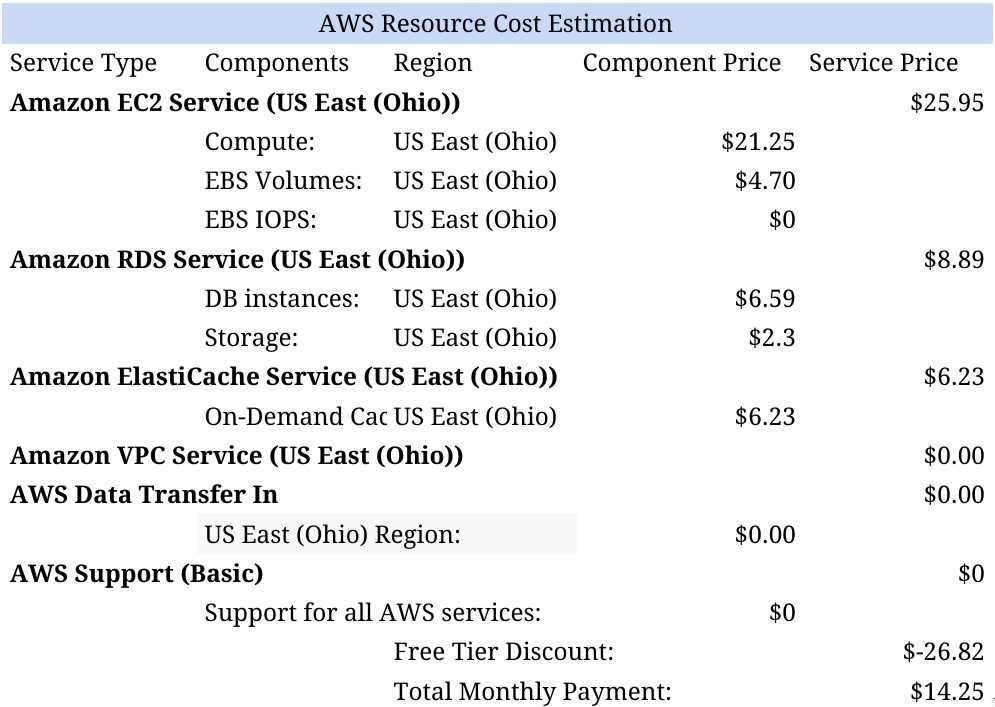
\includegraphics[width=12cm,height=8cm,keepaspectratio]{../media/crawler/aws-resource-cost-estimation.png}
  \caption{Whirlpool Hardware Cost Estimation on AWS}
  \label{fig:awscost}
\end{figure}

\noindent
With the free-tier in use, the total price is dropped almost by 50 \%. Under free tier, EC2 is limited to 750 hours/month which equates to approx. 24 hours/day for 30 days using only Linux, RHEL. Any combination of EBS (SSD/Magnetic) is 30 GiB. Amazon RDS again limited to 750 hours/month upto 20GB of general purpose SSD database
storage. Amazon ElasticCache - 750 hours. NAT Gateway is charged \$ 0.045 an hour. There is no charge for data transfer between cross-region multi-AZ as this implementation is 1 region, single AZ. Also, the data 
transfer into AWS cloud is free.

\pagebreak

\section{IAM and roles}\label{iamroles}
Showcase few IAM policies related to whirlpool project here.
\\
\\
\begin{figure}[h!]
  \centering
  
\includegraphics[width=14cm,height=14cm,keepaspectratio]{../media/crawler/iam_and_roles.png}
  \caption{Existing accounts and service role}
  \label{fig:iamroles}
\end{figure}

\noindent
I understood the use of roles because the way cloudformation works and how I interpret it - as a service it provisions other
services on behalf of user by assuming a service role. Use of service role in context of whirlpool project is given on a workout paper.
\\
the diagram
\\
A admin can create a service role with trust policy and attaching existing iam policies for whirlpool project and under 'resource'
section specifying a specific role cloudformation can assume. This way, a restricted IAM user whirlpooluser doesn't need to be give
permissions to create/modify/delete roles instead only list/describe/use roles. 

\pagebreak